\chapter{Aging-Aware Routing Algorithm System Design}

This section presents the system-level modeling framework and design choices used to enable reliability-aware routing in the NoC. The proposed approach integrates dynamic temperature variation, process variation, and aging models for EM and HCI directly into the routing decision process. These models are based on prior work in \cite{Clotho2015} and are combined with a reinforcement learning-based routing policy inspired by LARE \cite{LARE2023}.

Although other aging mechanisms, such as Bias Temperature Instability (BTI), also affect CMOS devices, they are not considered here. As discussed in \cite{Clotho2015}, BTI degradation is primarily associated with underutilized circuits and can be mitigated using techniques such as \textit{Use it or Lose it} \cite{Kim2013}. In contrast, EM and HCI are driven by switching activity and temperature, making them closely tied to traffic patterns and more appropriate for routing-level optimization.

Unlike conventional routing algorithms that optimize only performance metrics such as latency and throughput, this framework incorporates device-level reliability into routing decisions. Temperature and utilization are modeled as dynamic runtime inputs, while process variation is treated as a static parameter determined during initialization.

\section{Dynamic Temperature Variation}

Temperature is one of the primary factors governing the rate of both EM and HCI induced aging, and is therefore modeled explicitly as a dynamic runtime parameter. In a CMP, temperature is not spatially uniform. Instead, it varies across the die due to non-uniform activity in the processing and memory resources, which arises from application mapping, workload imbalance, and differences in instruction behavior. Following the modeling approach used in Clotho \cite{Clotho2015}, the chip is partitioned into an $n \times n$ grid of equal-area tiles. Each tile represents a thermal region containing one processing core, its associated cache resources, and the locally connected router with its nearest-neighbor bidirectional links. Within each tile, temperature is assumed to be uniform, while different tiles may exhibit different temperatures. This assumption is justified by the observation that the NoC contributes only a relatively small fraction of the total chip power budget, and that this power is spatially distributed across the die rather than concentrated in a small number of locations. Consequently, the dominant source of thermal variation is taken to be the computational activity of the processing elements, while the routers are treated as thermally coupled to the tiles that contain them \cite{Clotho2015}.

\begin{figure}[ht]
    \centering
    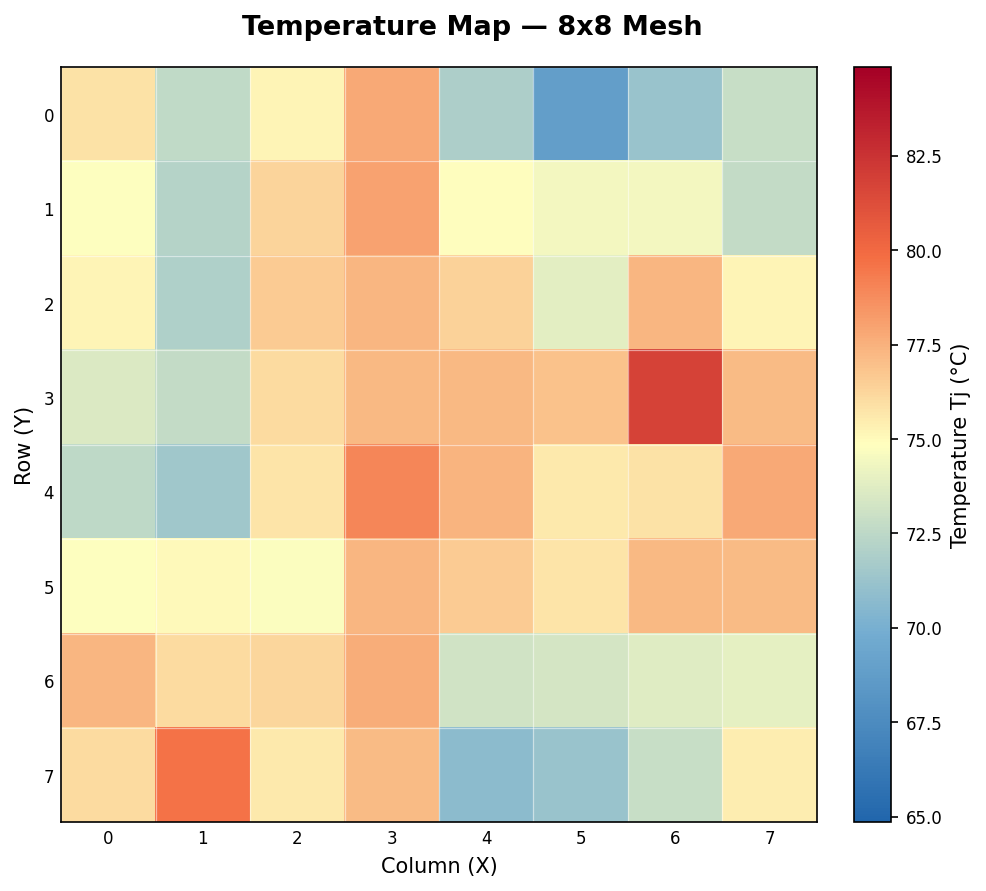
\includegraphics[width=0.95\linewidth]{body_chapters/chap_3/figs/temperature_map.png}
    \caption[Per-router temperature map]{Example spatial mapping of temperature across the NoC. The map reflects the combination of spatially correlated thermal variation.}
    \label{fig:temp_maps}
\end{figure}

Temperature is modeled as a slowly varying parameter rather than as a quantity that changes every cycle. In Clotho, the absolute values of the temperature map are updated every $10^7$ cycles in order to emulate the gradually changing thermal behavior of a running CMP, consistent with prior observations that on-chip temperature sensing and thermal evolution occur over millisecond-scale intervals rather than cycle-by-cycle timescales \cite{Clotho2015}. The same assumption is adopted here. Accordingly, the temperature map is periodically refreshed every $10^7$ cycles, allowing the routing algorithm to respond to long-term changes in the thermal profile without introducing unnecessary per-cycle thermal recomputation. The temperature assigned to each tile is generated as part of a spatial temperature map spanning the range of 65$^\circ$C to 85$^\circ$C, consistent with the range used in Clotho \cite{Clotho2015}. In implementation, these values are generated using a random but spatially correlated distribution so that neighboring tiles tend to exhibit similar thermal behavior. Figure \ref{fig:temp_maps} illustrates an example of such a temperature map. This per-tile temperature information is then used directly by the EM and HCI aging models. Since both failure mechanisms accelerate at higher temperatures, tiles operating at elevated temperature accumulate wear more rapidly than cooler tiles under otherwise similar activity conditions.

\section{Process Variation}

Process variation (PV) arises from fabrication-time imprecision and results in deviations of transistor parameters from their nominal values. As CMOS technology scales, these variations become more pronounced and introduce spatial non-uniformity in device characteristics across the chip. In the context of NoC reliability, PV plays an important role in modulating aging behavior, particularly for HCI, where transistor-level characteristics directly influence degradation rates \cite{Clotho2015}.

Following the Clotho model, PV is captured by considering variations in two key transistor parameters: the threshold voltage ($V_{th}$) and the effective gate length ($L_{eff}$). For each router, these parameters are modeled as:
\begin{equation}
V_{th} = V_{th0} + \Delta V_{th}, \quad V_{th0} = 179\ \text{mV}
\end{equation}
\begin{equation}
L_{eff} = L_{eff0} + \Delta L_{eff}, \quad L_{eff0} = 14.4\ \text{nm}
\end{equation}

The deviations $\Delta V_{th}$ and $\Delta L_{eff}$ are composed of two independent components:
\begin{equation}
\Delta V_{th} = \Delta V_{th,rand} + \Delta V_{th,sys}
\end{equation}
\begin{equation}
\Delta L_{eff} = \Delta L_{eff,rand} + \Delta L_{eff,sys}
\end{equation}

Systematic variation represents spatially correlated deviations caused by layout-dependent and process-wide effects. Neighboring regions of the chip tend to exhibit similar variation values. As in Clotho, systematic variation is modeled using a multivariate normal distribution with a spherical spatial correlation structure. The correlation between two regions depends only on their Euclidean distance $r$:
\begin{equation}
\rho(r) =
\begin{cases}
1 - \frac{3r}{2\phi} + \frac{r^3}{2\phi^3}, & r \leq \phi \\
0, & r > \phi
\end{cases}
\end{equation}
where $\phi$ represents the correlation range expressed as a fraction of the die length. In this work, $\phi = 0.5$, meaning that routers separated by more than half the die are effectively uncorrelated. Within a single region, variation is fully correlated ($\rho(0) = 1$), while distant regions exhibit no correlation \cite{Clotho2015}.

Random variation, in contrast, is uncorrelated and occurs at a much finer granularity, reflecting device-level fluctuations such as dopant variation. Both random and systematic components are assumed to follow normal distributions with zero mean. Since these components are independent, the total variation also follows a normal distribution with:
\begin{equation}
\sigma_{total} = \sqrt{\sigma_{rand}^2 + \sigma_{sys}^2}
\end{equation}

The parameter values used in this work are taken directly from Clotho and are summarized as follows:
\begin{itemize}
    \item For $V_{th}$: $\sigma_{rand} = 6.3\%$, $\sigma_{sys} = 6.3\%$
    \item For $L_{eff}$: $\sigma_{rand} = 3.2\%$, $\sigma_{sys} = 3.2\%$
    \item Correlation range: $\phi = 0.5$
\end{itemize}

Process variation is treated as a static property determined at fabrication time. Accordingly, the values of $V_{th}$ and $L_{eff}$ are generated once during initialization and remain constant throughout execution. In the implemented model, each router is assigned a fixed pair of $(V_{th}, L_{eff})$ values, which are stored and used throughout the simulation.

To visualize the spatial effect of process variation across the NoC, Figure \ref{fig:pv_maps} illustrates example per-router maps of the generated threshold voltage and effective gate length values. Since the systematic component is spatially correlated, neighboring routers tend to exhibit similar deviations, producing smooth regional variation rather than entirely independent fluctuations. The random component is then superimposed locally, yielding the final per-router values used in the model. Since process variation is not uniform across the chip, different routers may begin operation with different intrinsic susceptibility to HCI-induced degradation.

\begin{figure}[ht]
    \centering
    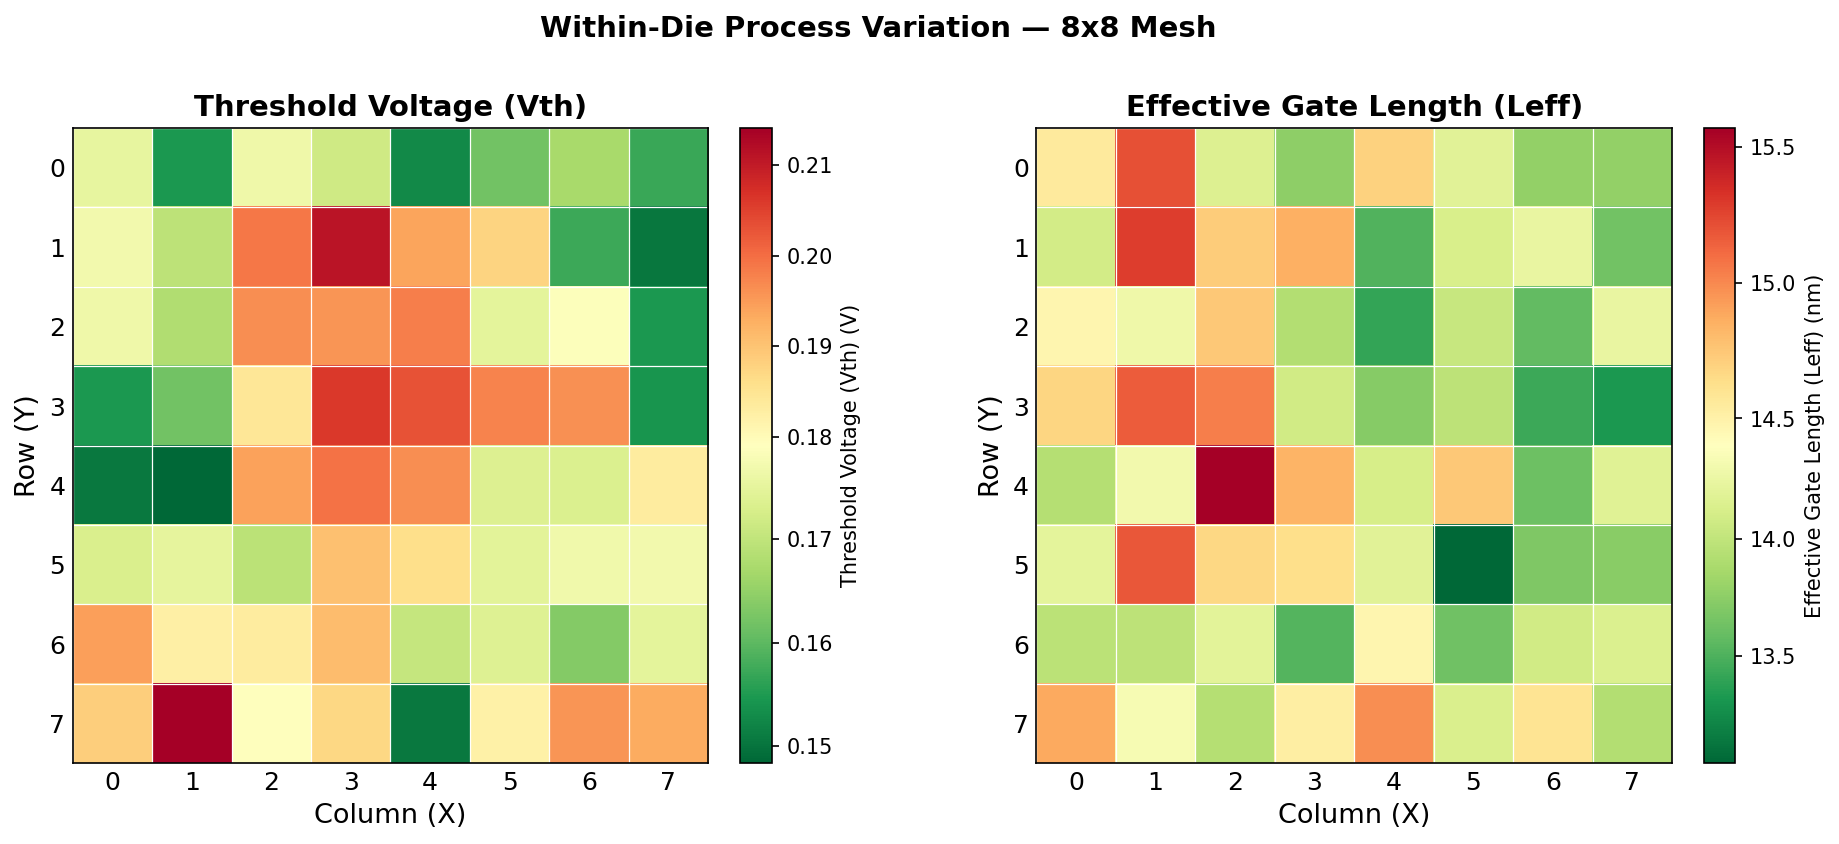
\includegraphics[width=1\linewidth]{body_chapters/chap_3/figs/process_variation_map.png}
    \caption[Per-router process variation maps]{Example spatial mapping of process variation across the NoC: (left) threshold voltage, $V_{th0} + \Delta V_{th}$, and (right) effective gate length, $L_{eff0} + \Delta L_{eff}$, for all routers in the mesh. The maps reflect the combination of spatially correlated systematic variation and uncorrelated random variation applied at initialization.}
    \label{fig:pv_maps}
\end{figure}

The resulting per-router values of $V_{th}$ and $L_{eff}$ are subsequently used to compute the substrate current ($I_{sub}$), which serves as an intermediate quantity in the HCI aging model. Since PV is static and all other parameters involved in this computation are technology constants, $I_{sub}$ can be precomputed once at initialization. The computation proceeds as follows:

\begin{equation}
V_{dsat} = \frac{(V_{gs} - V_{th}) \cdot L_{eff} \cdot E_{cr}}{(V_{gs} - V_{th}) + L_{eff} \cdot E_{cr}}
\end{equation}

where $V_{gs}$ is the gate-to-source voltage, $V_{th}$ is the threshold voltage, and $E_{cr}$ denotes the critical electric field associated with velocity saturation.

\begin{equation}
E_m = \frac{V_{ds} - V_{dsat}}{\sqrt{3 t_{ox} x_j}}
\end{equation}

where $V_{ds}$ denotes the drain-to-source voltage and $V_{dsat}$ corresponds to the voltage at the channel pinch-off point. The term $\sqrt{3 t_{ox} x_j}$ represents a characteristic length associated with the effective thickness of the pinch-off region in the transistor channel. For typical CMOS technologies, this length falls within the range $\sqrt{100\ \text{nm}}$ to $\sqrt{300\ \text{nm}}$.

\begin{equation}
I_{sub} = C_2 \cdot I_{ds} \cdot \exp\left(\frac{-\phi_i}{q \lambda_e E_m}\right)
\end{equation}

where $C_2$ is a proportionality constant, $I_{ds}$ is the drain current, $\phi_i$ denotes the minimum energy required for a hot electron to initiate impact ionization, $q$ is the elementary charge, $\lambda_e$ is the mean free path of hot electrons, and $E_m$ is the electric field in the channel.

All parameters other than $V_{th}$ and $L_{eff}$ are treated as technology-dependent constants and are fixed based on values reported in prior work. The resulting $I_{sub}$ value is stored as a single scalar per router, eliminating the need for repeated evaluation of the above expressions during runtime. The precomputed $I_{sub}$ is later used in the HCI aging model to determine degradation rates as a function of switching activity and temperature.

\section{Aging Models}

\subsubsection{Electromigration (EM)}

Electromigration (EM) is a wearout mechanism in which momentum transfer from conducting electrons causes gradual displacement of metal ions in interconnect wires. Under sustained high current density, this ion migration leads to the formation of voids and hillocks, eventually resulting in open- or short-circuit failures. As technology scales and interconnect dimensions shrink, current densities increase, making EM a critical reliability concern in modern NoCs \cite{Clotho2015}.

The lifetime of an interconnect under EM stress is commonly modeled using Black's equation:
\begin{equation}
MTTF_{EM} = A_{EM} J^{-n} \exp\left(\frac{E_{a,EM}}{kT}\right)
\end{equation}
where $J$ is the current density, $n$ is an empirical exponent (typically close to 2), $E_{a,EM}$ is the activation energy, $T$ is temperature, and $k$ is Boltzman's constant.

In NoC interconnects, current density is closely related to switching activity. As traffic increases, links are exercised more frequently, leading to a higher rate of current flow through the interconnect. Long router-to-router links tend to carry a larger share of traffic and exhibit higher effective current density compared to shorter intra-router wires. As a result, these links are more susceptible to electromigration-induced degradation.

Following \cite{Clotho2015}, current density is expressed in terms of link switching activity:
\begin{equation}
J \propto \alpha_{link}
\end{equation}

Substituting this relationship into Black's equation yields a simplified proportional model:
\begin{equation}
MTTF_{EM}(\alpha_{link}, T) \propto \alpha_{link}^{-2} \cdot \exp\left(\frac{E_{a,EM}}{kT}\right)
\end{equation}

The switching activity $\alpha_{link}$ is derived from link utilization:
\begin{equation}
\alpha_{link} = 0.5 \times U_{link}
\end{equation}
which assumes random data patterns, where each bit has a 50\% probability of switching.

In this work, EM is modeled at the granularity of individual links. A proportional MTTF value is computed for each link based on its runtime utilization and temperature. These values are updated periodically as network conditions evolve.

A key characteristic of this model is its quadratic dependence on switching activity. As a result, EM is highly sensitive to traffic distribution. Even modest reductions in link utilization can produce significant improvements in lifetime. This makes EM particularly responsive to routing-level load balancing, where redistributing traffic away from heavily utilized links can substantially reduce localized wear.

\subsubsection{Hot-Carrier Injection (HCI)}

Hot-carrier injection (HCI) is a transistor-level aging mechanism caused by high-energy carriers that become trapped in the gate oxide during switching. Over time, this leads to a gradual increase in threshold voltage ($V_{th}$), which slows transistor switching speed and degrades circuit performance. In NoC routers, this degradation is most critical along timing-critical paths, where increased delay can eventually result in timing violations and system failure \cite{Clotho2015}.

The lifetime of a device under HCI stress can be expressed as:
\begin{equation}
MTTF_{HCI}^{DC} = A_{HCI} (I_{sub})^{-N} \exp\left(\frac{E_{a,HCI}}{kT}\right)
\end{equation}
where $I_{sub}$ is the substrate current during stress, $N$ is an empirical exponent (approximately 1.5), and $E_{a,HCI}$ is the activation energy.

Since HCI degradation occurs during switching events, its impact under dynamic operation is proportional to switching activity. Incorporating this effect yields:
\begin{equation}
MTTF_{HCI}^{AC}(\alpha_{router}, T) \propto \frac{(I_{sub})^{-N}}{\alpha_{router}} \cdot \exp\left(\frac{E_{a,HCI}}{kT}\right)
\end{equation}

Here, $\alpha_{router}$ represents the switching activity along the router’s critical path. Based on empirical observations in \cite{Clotho2015}, this activity is related to router utilization by:
\begin{equation}
\alpha_{router} = 0.1 \times U_{router}
\end{equation}
reflecting that only a subset of flits (primarily header flits) exercise the critical path.

Unlike EM, HCI is strongly influenced by process variation. Variations in threshold voltage ($V_{th}$) and effective gate length ($L_{eff}$) affect the substrate current $I_{sub}$, which in turn determines degradation rate. As described in the previous section, $I_{sub}$ is computed per router as a function of these parameters and treated as a static quantity throughout execution.

Combining these effects yields the final HCI model used in this work:
\begin{equation}
MTTF_{HCI,PV} \propto \frac{(I_{sub}(V_{th}, L_{eff}))^{-N}}{\alpha_{router}} \cdot \exp\left(\frac{E_{a,HCI}}{kT}\right)
\end{equation}

This model captures both dynamic and static sources of degradation. The switching activity and temperature introduce time-varying stress, while process variation establishes a fixed baseline reliability for each router. As a result, routers with unfavorable $(V_{th}, L_{eff})$ values begin operation with reduced timing margin and are inherently more vulnerable to HCI-induced degradation.

Compared to EM, HCI exhibits a weaker dependence on switching activity due to its linear relationship with $\alpha_{router}$. Consequently, while traffic redistribution can still improve HCI lifetime, its impact is less pronounced than in the case of EM.

\subsubsection{Utilization of Lifetime Models}

The EM and HCI models described above are used to guide routing decisions and evaluate system reliability. During routing, the MTTF of candidate next-hop links and routers is computed using current utilization and temperature values. These MTTF estimates are normalized relative to the network state and used to define the reward signal for the reinforcement learning policy. Routing decisions are therefore biased toward paths that traverse components with higher estimated lifetime.

Throughout simulation, MTTF values are updated periodically as utilization statistics and temperature maps are refreshed. This enables the system to track the evolution of wear across all network components under dynamic traffic conditions. At the end of simulation, the final MTTF values of all routers and links are collected. The system lifetime is defined by the most degraded component, reflecting the fact that failure of a single critical link or router can render the network unusable.

To compare routing algorithms, the acceleration factor (AF) is used as a relative lifetime metric:
\begin{equation}
AF_{EM} = \frac{MTTF_{EM}|_{RL}}{MTTF_{EM}|_{DOR}}, 
\quad
AF_{HCI} = \frac{MTTF_{HCI,PV}|_{RL}}{MTTF_{HCI,PV}|_{DOR}}
\end{equation}

Since both configurations share identical process variation and technology parameters, unknown constants and the precomputed $I_{sub}$ cancel out in the ratio. As a result, the acceleration factor depends only on runtime variables such as utilization and temperature.

\section{Reinforcement Learning-Based Routing Policy}

Reinforcement learning (RL) is a learning framework in which an agent interacts with an environment to learn a policy that maximizes long-term cumulative reward. At each decision step, the agent observes the current state $s$, selects an action $a$, and receives a reward $r$ based on the outcome of that action. The system then transitions to a new state $s'$, and the process repeats. Over time, the agent improves its decision-making by learning from these interactions. Figure~\ref{fig:RL_framework} illustrates this agent–environment interaction model.

\begin{figure}[ht]
  \centering
  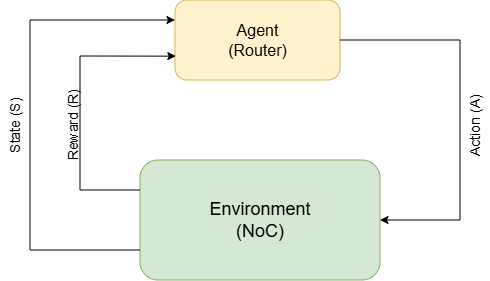
\includegraphics[width=0.7\linewidth]{body_chapters/chap_3/figs/RL.png}
  \caption[Reinforcement Learning Framework]{Agent–environment interaction in reinforcement learning.}
  \label{fig:RL_framework}
\end{figure}

In this work, we adopt Q-learning, a value-based RL method. Q-learning estimates the expected cumulative reward of taking an action $a$ in a state $s$, represented by the Q-value function $Q(s,a)$. The optimal policy is obtained by selecting actions that maximize this value.

The Q-values are updated iteratively using the Bellman equation:

\begin{equation}
Q(s,a) \leftarrow Q(s,a) + \alpha \left[ r + \gamma \max_{a'} Q(s',a') - Q(s,a) \right]
\end{equation}

where $\alpha$ is the learning rate and $\gamma$ is the discount factor. The term inside the brackets is the temporal-difference (TD) error, which measures how well the current estimate matches observed outcomes.

In the context of NoCs, routing decisions can be formulated as a sequential decision-making problem, where each router selects the next-hop direction for a packet based on local network conditions. Each router is modeled as an independent RL agent, and routing corresponds to selecting an action that maximizes long-term reward. Direct application of tabular Q-learning, however, is impractical in NoCs due to the large state-action space, which grows rapidly with network size. This leads to excessive storage requirements and slow convergence, commonly referred to as the curse of dimensionality. To address this limitation, this work adopts a linear function approximation approach inspired by LARE \cite{LARE2023}, where Q-values are represented using a compact feature-based model instead of a lookup table.

\subsubsection{State Representation}

Routing decisions are made at each router when multiple minimal paths are available. Instead of representing the state explicitly, each state-action pair $(s,a)$ is encoded using a feature vector $\phi(s,a)$:

\begin{equation}
\phi(s,a) = [f_0, f_1, f_2, f_3, f_4, f_5, f_6, f_7, f_8]
\end{equation}

where:
\begin{itemize}
    \item $f_0$: Bias term (constant 1)
    \item $f_1$: Destination router ID
    \item $f_2$: Current router ID
    \item $f_3$: Distance traveled in hops from source to current router
    \item $f_4$: Remaining distance to destination
    \item $f_5$: EM MTTF of candidate link
    \item $f_6$: HCI MTTF of candidate router
    \item $f_7$: Output port congestion level
    \item $f_8$: Encoded input port direction
\end{itemize}

This representation allows the agent to incorporate both performance related and reliability related information into routing decisions.

\subsubsection{Q-Value Function}

To reduce hardware overhead, the Q-value is approximated using a linear function:

\begin{equation}
Q(s,a) = \theta_0 \cdot f_0 + \theta_1 \cdot f_1 + \theta_2 \cdot f_2 + \theta_3 \cdot f_3 + \theta_4 \cdot f_4 + \theta_5 \cdot f_5 + \theta_6 \cdot f_6 + \theta_7 \cdot f_7 + \theta_8 \cdot f_8
\end{equation}

where $f_i$ represents the $i$-th feature in the state-action vector, and $\theta_i$ is the corresponding learned coefficient. Each coefficient captures the contribution of its feature toward the estimated long-term reward.

This approach eliminates the need to store a full Q-table, reducing memory requirements and enabling scalable implementation at the router level, while still allowing the model to capture relationships between features and long-term reward.

\subsubsection{Action Selection Policy}

An $\epsilon$-greedy policy is used to balance exploration and exploitation:

\begin{equation}
a =
\begin{cases}
\text{random action}, & \text{with probability } \epsilon \\
\arg\max_a Q(s,a), & \text{otherwise}
\end{cases}
\end{equation}

The action space consists of minimal routing directions (e.g., horizontal and vertical moves in a mesh topology).

\subsubsection{Reward Function}

The reward function is designed to jointly capture reliability and performance objectives. It combines normalized aging metrics with congestion information:

\begin{equation}
R = 0.7 \cdot \text{MTTF}_{score} - 0.3 \cdot \text{cong}_{norm}
\end{equation}

The reliability component is defined as:
\begin{equation}
\text{MTTF}_{score} = C_{EM} \cdot EM_{norm} + C_{HCI} \cdot HCI_{norm}
\end{equation}

The EM and HCI values are normalized across candidate actions:
\begin{equation}
EM_{norm} = \frac{MTTF_{EM}}{\max(MTTF_{EM}^{(h)}, MTTF_{EM}^{(v)})}
\end{equation}

\begin{equation}
HCI_{norm} = \frac{MTTF_{HCI}}{\max(MTTF_{HCI}^{(h)}, MTTF_{HCI}^{(v)})}
\end{equation}

where the superscripts $(h)$ and $(v)$ denote the horizontal and vertical candidate next hops, respectively.

To dynamically emphasize the more critical aging mechanism, adaptive weights are computed using:

\begin{equation}
C(x) =
\frac{\exp\left(8 \cdot \frac{x - x_{min}}{x_{max} - x_{min}}\right) - \exp(-8)}
{1 - \exp(-8)}
\end{equation}

where $x \in \{MTTF_{EM}, MTTF_{HCI}\}$, and $x_{max}$ and $x_{min}$ are the maximum and minimum values among candidate actions. The weights are then defined as:

\begin{equation}
C_{EM} = C(MTTF_{EM}), \quad C_{HCI} = C(MTTF_{HCI})
\end{equation}

The congestion term reflects the load on the output port:
\begin{itemize}
    \item Low congestion: $0$
    \item Medium congestion: $0.5$
    \item High congestion: $1.0$
\end{itemize}

This formulation encourages the routing policy to prefer paths that both reduce congestion and avoid highly stressed components.

\subsubsection{Update Rule}

The parameter vector $\theta$ is updated using temporal-difference learning. First, the TD error is computed:

\begin{equation}
\delta = R + \gamma \max_{a'} Q(s', a') - Q(s,a)
\end{equation}

The parameters are then updated as:

\begin{equation}
\theta \leftarrow \theta + \alpha \cdot \delta \cdot \phi(s,a)
\end{equation}

This update adjusts the model parameters in the direction that reduces the discrepancy between predicted and observed rewards, allowing the routing policy to improve over time.

\section{Deadlock Avoidance}

Adaptive routing algorithms, including the proposed RL-based routing policy, do not inherently guarantee deadlock freedom \cite{LARE2023}. Since routing decisions are made dynamically based on network conditions, packets may acquire resources in different orders, potentially leading to cyclic dependencies. To understand how deadlock arises and how it can be prevented, it is first necessary to examine the underlying router microarchitecture.

\subsubsection{Router Microarchitecture}

A typical NoC router employs virtual channel (VC) flow control to efficiently utilize network resources. As shown in Figure~\ref{fig:router_arch}, each router consists of input ports with associated buffers, a routing unit, a switch allocator, a crossbar, and output ports.

\begin{figure}[ht]
    \centering
    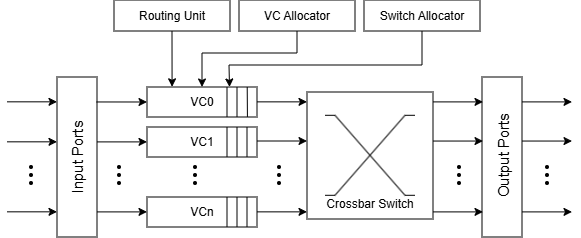
\includegraphics[width=0.95\linewidth]{body_chapters/chap_3/figs/router.png}
    \caption[NoC Router Microarchitecture]{Router microarchitecture based on virtual channel flow control.}
    \label{fig:router_arch}
\end{figure}

Incoming packets arrive at an input port and are stored in input buffers organized as multiple virtual channels. Each VC maintains a separate queue of flits, allowing multiple packets to share the same physical channel without blocking each other. When a packet reaches the head of a VC, the routing unit determines the set of candidate output ports based on the routing algorithm. The packet then requests access to a downstream VC at the next router. Once a downstream VC is successfully allocated, the packet competes for access to the crossbar through the switch allocator. If granted, the packet is forwarded through the crossbar to the selected output port and transmitted to the next router. This process repeats at each hop, resulting in a sequence of resource acquisitions: input VC, downstream VC, switch allocation, and output link traversal.

\subsubsection{Deadlock Formation}

The staged allocation of resources creates dependencies between packets across routers. A packet occupying a VC at one router may be blocked while waiting for a downstream VC at the next router. If that downstream VC is already occupied by another packet, the dependency extends further along the network. Deadlock occurs when a set of packets forms a cyclic dependency, where each packet holds a resource while waiting for another resource held by another packet in the cycle.

\begin{figure}[ht]
    \centering
    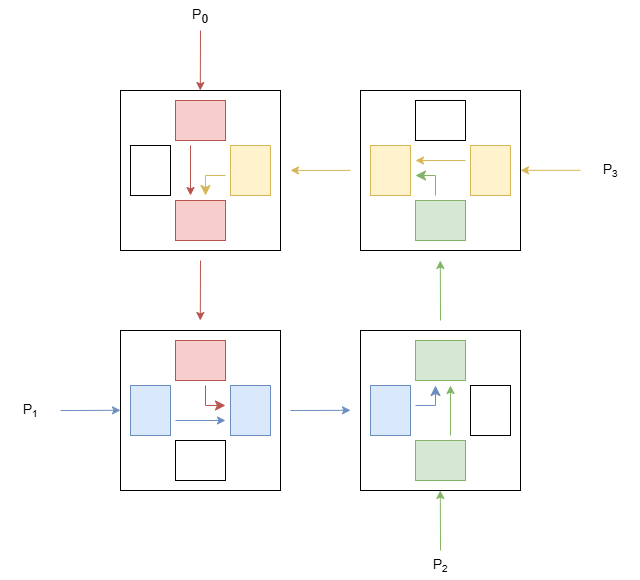
\includegraphics[width=0.95\linewidth]{body_chapters/chap_3/figs/deadlock.png}
    \caption[Deadlock Formation]{Example of cyclic resource dependency leading to deadlock in a mesh NoC.}
    \label{fig:deadlock_cycle}
\end{figure}

In a 2D mesh, such cycles can occur when packets routed in different directions occupy VCs in neighboring routers while waiting for each other's downstream resources, forming a closed loop. Since none of the packets can release their current resources until they acquire the next one, no forward progress is possible. This is illustrated in Figure~\ref{fig:deadlock_cycle}, where packets $P_0$, $P_1$, $P_2$, and $P_3$ form a cycle of dependencies across four routers. Each packet is waiting for a buffer in the downstream router that is currently being occupied by another packet in the cycle, resulting in a situation where no packet can proceed and the system is effectively stalled.

Adaptive routing increases the likelihood of such cycles because it allows packets to dynamically select different paths. Unlike deterministic routing, which enforces a strict ordering of channel acquisition, adaptive routing introduces flexibility that can lead to arbitrary dependency patterns and potential deadlock.

\subsubsection{Deadlock Avoidance Using Escape Virtual Channels}

To guarantee deadlock freedom, this work adopts an escape virtual channel mechanism based on Duato's theory \cite{Duato1993}. The key idea is to reserve a subset of network resources that follow a strictly deadlock-free routing function, ensuring that at least one acyclic path is always available.

In this implementation, one virtual channel (VC0) is designated as the escape channel and is restricted to deterministic dimension-order (XY) routing. Since XY routing enforces a strict ordering of channel acquisition and is provably deadlock-free, any packet assigned to this channel is guaranteed forward progress. All remaining virtual channels are allowed to use the RL-based adaptive routing policy. If a packet cannot safely proceed using adaptive routing, it can transition to the escape VC and continue using XY routing. This mechanism ensures that cyclic dependencies are avoided while preserving the flexibility of adaptive routing for the majority of traffic.

% \section{Tables}

% Tables can be placed with the \textbf{\textbackslash table} environment. The same instructions for the figures apply here; use the \textbf{\textbackslash label} command often

% \begin{center}
%   \begin{table}[h]
%     \centering
%     \begin{tabular}{l c l c}
%     \hline
%     Layer Type & Size & Activation & Regularization\\
%     \hline
%     Flatten& $30 \times 30 \times 3$ &ReLU & ---\\
%     Dense & 4096 & ReLU & 10\% Dropout\\
%     Dense & 2048 & ReLU & 10\% Dropout\\
%     Dense & 1024 & ReLU & 10\% Dropout\\
%     Dense & 1024 & ReLU & --- \\
%     Dense & 6 & Softmax & --- \\
%     \hline
%     \end{tabular}
%     \caption[Short Caption for List of Tables.]{Long caption to appear in the body of the text with the table.}
%     \label{tab:ModelArchitecture}
%   \end{table}
% \end{center}
